\section{The Scoring Reducer}
\label[appendix]{app:reducer}
\label[appendix]{sec:design}

This section specifies the general reducer that verify-then-vote's selector $\mathrm{sel}$ runs on (\paperref{main-paper rule}): how answers become typed claims, how conflicts are detected, how candidates are scored, and when its tie-break provably cannot change correctness. On OVERTURN the simplest selector, plurality among verified answers, matches the scored one on accuracy (\paperref{main-paper passage controls}); the scoring reducer is the general form for open-ended claims with many slots per answer.

\subsection{Pipeline and running example}
\label[subappendix]{sec:pipeline}

\begin{figure}[t]
  \centering
  % The arbitration boundary (coordinates on a 680 x 200 grid).
\begin{tikzpicture}[x=0.0235cm,y=-0.0235cm,font=\footnotesize,
    box/.style={draw,thin,minimum height=38*0.0235cm,inner sep=1pt,align=center},
    key/.style={box,fill=blue!8,line width=0.9pt},
    grey/.style={box,fill=black!5},
    arr/.style={-{Stealth[length=4pt]},thin}]
  \node[anchor=west,text=black!65] at (10,10) {artifact production (stochastic; every output recorded)};
  \node[grey,minimum width=100*0.0235cm] (ag) at (60,39) {agents\\(free text)};
  \node[box,minimum width=95*0.0235cm]  (p1) at (177.5,39) {P1 normalize};
  \node[box,minimum width=95*0.0235cm]  (p2) at (292.5,39) {P2 lower};
  \node[box,minimum width=95*0.0235cm]  (p3) at (407.5,39) {P3 validate};
  \node[key,minimum width=195*0.0235cm] (seal) at (572.5,39) {SEAL: artifact set $A$\\canonical form, root hash};
  \draw[arr] (ag) -- (p1);
  \draw[arr] (p1) -- (p2);
  \draw[arr] (p2) -- (p3);
  \draw[arr] (p3) -- (seal);
  % reducer frame
  \draw[thin,dash pattern=on 5pt off 4pt] (135,92) rectangle (670,190);
  \node[anchor=west,text=black!65,font=\scriptsize] at (140,180) {reducer $C(A, P)$: pure, reads only $A$ and $P$};
  \node[anchor=east,text=black!65,font=\scriptsize] at (665,180) {certificate = $H$(root, policy hash, admitted ids)};
  \node[box,minimum width=100*0.0235cm] (p4) at (200,137) {P4 conflicts};
  \node[box,minimum width=100*0.0235cm] (p5) at (320,137) {P5 select};
  \node[box,minimum width=100*0.0235cm] (p6) at (440,137) {P6 commit};
  \node[grey,minimum width=150*0.0235cm] (out) at (585,137) {admitted ids\\+ certificate};
  \node[key,minimum width=105*0.0235cm] (pol) at (62.5,137) {policy $P$\\frozen, hashed};
  \draw[arr] (seal.south) -- (p4.north);
  \draw[arr] (p4) -- (p5);
  \draw[arr] (p5) -- (p6);
  \draw[arr] (p6) -- (out);
  \draw[arr] (pol) -- (p4);
\end{tikzpicture}

  \caption{The arbitration boundary. Passes P1--P3 produce artifacts and may involve models; their outputs are sealed into $A$. Passes P4--P6 form the reducer $C$, which reads only $A$ and $P$.}
  \label{fig:boundary}
\end{figure}

\Cref{fig:boundary} shows the six passes. Intent normalization (P1) produces the goal and criteria; if it uses a model, its output is an artifact like any other. Lowering (P2) is rule-based: clause segmentation, a 125-entry hedge lexicon for confidence, a rule cascade that extracts triples with polarity, evidence-marker patterns, and a round-trip reconstruction that grades each contribution HIGH, MEDIUM, or LOW. Validation (P3) drops contributions without a triple, rejects synthesis contributions (\cref{sec:output}), orders the rest canonically, and removes duplicate identifiers. The reducer then detects conflicts (P4), selects (P5), and commits (P6).

Before the full example, we define the \emph{deadband}: scores close enough to the highest score are treated as tied for a separate selection step. With a width of 0.05 and a top score of 0.60, a score of 0.58 enters that step, whereas 0.50 does not. The implementation uses quantized scores and a strict inequality, specified in \cref{sec:selection,sec:implementation}.

A small example shows the path. Asked for the capital of Australia, five agents answer in arrival order A--E: A says Sydney without evidence; B and C say Canberra, citing Wikipedia and the CIA World Factbook; D and E say Canberra without citations. All state confidence 0.8 under the default calibration factor 0.5. Because \code{has\_capital} is functional, the five triples compete for one slot. The default policy scores them A 0.480, B 0.553, C 0.566, D 0.518, and E 0.530: citations add 0.06 and arrival order up to 0.05. C scores highest, but B, D, and E lie within the deadband of width 0.05 below it, so the tie-breaker runs over the four Canberra claims and selects B. Sydney and the other Canberra copies are rejected and kept in the audit record. Since every deadband candidate is correct, the tie-break decides only which copy is admitted. Yet the weakest correct claim (0.518) leads the incorrect one (0.480) by less than 0.05, so the separation condition of \cref{sec:selection} fails even though the selection is safe: separation is sufficient rather than necessary.

\subsection{Claims and slots}
\label[subappendix]{sec:slots}

A contribution carries an agent identifier, a kind (ASSERTION or CRITIQUE), a canonical triple (subject, predicate, object, polarity AFFIRM or NEGATE), a confidence, evidence items, its raw text, and its lowering grade. Its identifier is the first 128 bits of a SHA-256 hash over a canonical serialization of exactly these fields plus a scheme tag. The arrival index is excluded, since ingestion rather than the agent assigns it, but the root hash covers it. Sealing accepts only identifiers that equal their content hash, and replay re-checks every one, so editing a claim changes its identity. Binding the agent identifier into the hash gives two agents with identical text distinct identifiers; the agent identifier is an unauthenticated label.

Slots define what a conflict is, and their key depends on predicate arity. A \emph{functional} predicate such as \code{has\_capital} admits one object per subject, so its key is (subject, predicate) and different objects compete. A \emph{non-functional} predicate such as \code{uses} admits many, so its key includes the normalized object and compatible claims occupy separate slots, within which AFFIRM and NEGATE still conflict. Keying by (subject, predicate) alone would make ``TCP uses sequence numbers'' and ``TCP uses acknowledgments'' compete for one occupant. Arity alone leaves exclusive objects of a non-functional predicate, such as a two-way versus a three-way handshake, indistinguishable from compatible ones, so the policy declares an \emph{exclusivity table} of object groups; a grouped object is keyed by its group, whose members compete. Conflict detection (P4) is thus a lookup over the declared arity and exclusivity tables (\paperref{main-paper limitations}).

\subsection{Output and provenance}
\label[subappendix]{sec:output}

The reducer's output is a set of contribution identifiers: the admitted/rejected partition over submitted ASSERTION contributions, plus each slot's members, scores, and winner. Commit (P6) admits each slot's winner and rejects the other members, which stay in the audit record; uncontested contributions are admitted unless they are critiques or LOW-graded, and a claim fewer than two agents asserted is flagged as uncorroborated. Because validation rejects SYNTHESIS contributions, and a property test checks that every admitted identifier is a submitted ASSERTION, provenance holds by construction: every output identifier names content some agent submitted. The reducer outputs identifiers rather than rendered text, and selection is embedding-free.
\subsection{Selection and its guarantees}
\label[subappendix]{sec:selection}

The question for this section is when a tie-breaker cannot change the correctness of the reducer's choice. The answer depends on the combined score rather than any one feature. For example, two HIGH-graded candidates identical except for evidence values of 0.90 and 0.80 differ in total score by $0.35(0.90-0.80)=0.035$ under the default evidence weight. That difference is smaller than the deadband width of 0.05, so both candidates proceed to the tie-break step. We now define all five score components and the conditions under which the deadband contains only correct candidates.

\paragraph{Scoring.} Each candidate $c$ has a feature vector $x(c) = (\textrm{ev}, \textrm{conf}, \textrm{cs}, \textrm{rec}, \textrm{ca}) \in [0,1]^5$ and a lowering factor $\lambda(c)$, with $\lambda = 1.0, 0.85, 0.5$ for HIGH, MEDIUM, and LOW. Its score is
\begin{equation*}
  \Score_w(c) = \lambda(c)\, w^\top x(c), \qquad w = (0.35,\ 0.20,\ 0.25,\ 0.05,\ 0.15) \textrm{ by default.}
\end{equation*}
\emph{Evidence} is $\textrm{ev}(c) = \min\bigl(1, \sum_e w_e\, t_e\, q_e\, r_e\, m_e\bigr)$: stated weight, a type weight (tool result 1.0 down to reasoning 0.3), a verification factor (0.40 for unverified citations), a reachability factor (0.75 if marked reachable, 0.45 if not), and a cross-reference multiplier from 0.9 to 1.2 that grows with the number of agents citing the source. By default this checks only that evidence exists; \cref{sec:evidence} adds whether it supports the claim. \emph{Confidence} is stated confidence times the agent's calibration factor. \emph{Critique survival} is $\max(0, 1 - \sum_k \textrm{severity}_k / 5)$ over NEGATE critiques of the claim's triple, capped per agent. \emph{Recency} is the rank of $\sigma$ in the conflict set, scaled to $[0, 1]$. \emph{Criterion alignment} is the fraction of acceptance criteria the claim matches lexically.

\paragraph{Deadband and tie-break.} When the top two quantized scores differ by less than $\delta = 0.05$, the reducer runs a Schulze widest-path election \citep{schulze2011new} over the \emph{deadband set} of candidates strictly within $\delta$ of the top, with each of the five features as a voter that prefers one candidate to another when its feature value is higher by more than an indifference threshold (0.01 by default); residual ties go to the earliest candidate in canonical order (lowest $\sigma$, then identifier). The policy offers order-free alternatives: zero recency weight, recency removed from the voters, residual ties ordered by identifier, a ``highest score, then canonical order'' tie-break, and value-level candidates. With the first three set, selection is independent of arrival order.

\paragraph{Why the margin must cover the total score.} One might require only that correct claims carry more evidence than incorrect ones by more than $\delta$. That condition leaves the tie-breaker exposed. Take two HIGH-graded candidates under the default weights with confidence 0.5, critique survival 1, and criterion alignment 1; the correct one has evidence 0.90 and arrived first, the incorrect one evidence 0.80 and arrived last. Their scores are
\begin{align*}
  \textrm{correct:}\quad & 0.35(0.90) + 0.20(0.5) + 0.25 + 0 + 0.15 = 0.815,\\
  \textrm{incorrect:}\quad & 0.35(0.80) + 0.20(0.5) + 0.25 + 0.05 + 0.15 = 0.830.
\end{align*}
The evidence gap is $0.10 > \delta$, yet both candidates fall in the deadband and the incorrect one scores higher (\cref{fig:evidence-gap}). The other four features and the lowering factor can outweigh any evidence gap, so a correct condition must be stated over the total score.

\begin{figure}[t]
  \centering
  % Why an evidence gap is not enough. The two points are the
% counterexample of Appendix B.4 (default weights, conf 0.5, cs 1, ca 1, HIGH):
%   correct:   ev 0.90, rec 0 -> 0.35*0.90 + 0.20*0.5 + 0.25 + 0    + 0.15 = 0.815
%   incorrect: ev 0.80, rec 1 -> 0.35*0.80 + 0.20*0.5 + 0.25 + 0.05 + 0.15 = 0.830
% Deadband: scores within 0.05 of the top score 0.830, i.e. [0.780, 0.830].
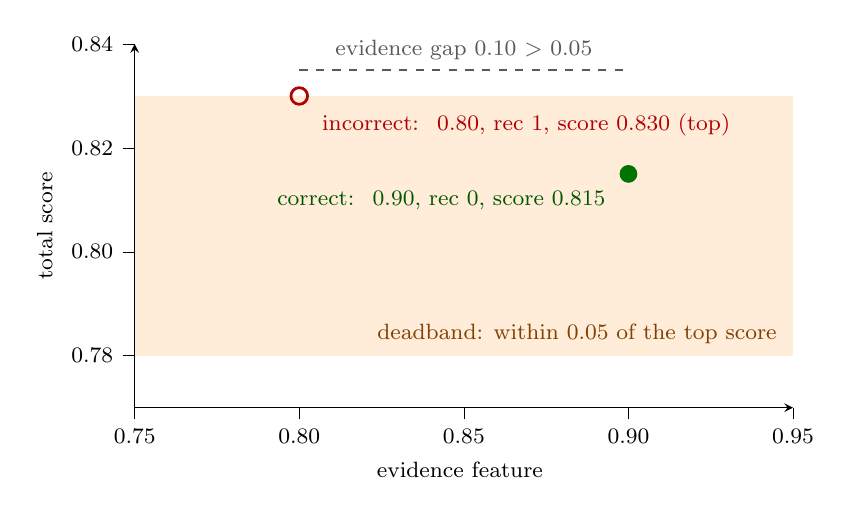
\begin{tikzpicture}
  \begin{axis}[
      width=0.82\linewidth, height=6.2cm,
      xmin=0.75, xmax=0.95, ymin=0.77, ymax=0.84,
      xtick={0.75,0.80,0.85,0.90,0.95},
      ytick={0.78,0.80,0.82,0.84},
      xticklabel style={/pgf/number format/.cd,fixed,fixed zerofill,precision=2},
      yticklabel style={/pgf/number format/.cd,fixed,fixed zerofill,precision=2},
      xlabel={evidence feature $\ev$}, ylabel={total score},
      axis lines=left, tick align=outside, tick style={black},
      font=\footnotesize, clip=false]
    \fill[orange!15] (axis cs:0.75,0.780) rectangle (axis cs:0.95,0.830);
    \node[anchor=south east,text=orange!50!black] at (axis cs:0.948,0.7805)
      {deadband: within 0.05 of the top score};
    \draw[dashed,black!65] (axis cs:0.80,0.8350) -- (axis cs:0.90,0.8350)
      node[midway,above,text=black!65] {evidence gap 0.10 $>$ 0.05};
    \addplot[only marks,mark=o,mark size=3pt,draw=red!70!black,line width=1pt]
      coordinates {(0.80,0.830)};
    \addplot[only marks,mark=*,mark size=3pt,color=green!45!black]
      coordinates {(0.90,0.815)};
    \node[anchor=north west,text=red!70!black] at (axis cs:0.804,0.8285)
      {incorrect: $\ev$ 0.80, rec 1, score 0.830 (top)};
    \node[anchor=north east,text=green!35!black] at (axis cs:0.896,0.8135)
      {correct: $\ev$ 0.90, rec 0, score 0.815};
  \end{axis}
\end{tikzpicture}

  \caption{Why an evidence gap is insufficient. The correct claim has more evidence, but recency lifts the incorrect claim above it; both lie inside the deadband, so the tie-breaker may pick either.}
  \label{fig:evidence-gap}
\end{figure}

\paragraph{Notation.} For a conflict set $S_k$ whose correct and incorrect classes $S_k^+$ and $S_k^-$ are both non-empty, and a pair $(c^+, c^-) \in S_k^+ \times S_k^-$, let $d(c^+, c^-) = \lambda(c^+)\,x(c^+) - \lambda(c^-)\,x(c^-) \in [-1,1]^5$, so that $\Score_w(c^+) - \Score_w(c^-) = w^\top d(c^+, c^-)$.

\begin{definition}[Score separation]
\label{def:separation}
$S_k$ is \emph{score-separated} under $w$ with margin $\delta \geq 0$ if $\Delta_w(S_k) = \min_{S_k^+} \Score_w - \max_{S_k^-} \Score_w > \delta$, equivalently if $w^\top d(c^+, c^-) > \delta$ for every pair.
\end{definition}

\begin{proposition}[Deadband homogeneity]
\label{prop:homogeneity}
If $S_k$ is score-separated under $w$ with margin $\delta \geq 0$, then (i) every maximizer of $\Score_w$ over $S_k$ is correct, and (ii) every member of the deadband set $D_\delta = \lbrace c : \Score_w(c) \geq \max \Score_w - \delta \rbrace$ is correct.
\end{proposition}

\begin{proof}
(i) If a maximizer $c^\star$ were incorrect, any correct $c^+$ would satisfy $\Score(c^+) > \Score(c^\star) + \delta \geq \Score(c^\star)$. (ii) Every incorrect $c^-$ has $\Score(c^-) < \min_{S_k^+}\Score - \delta \leq \max\Score - \delta$.
\end{proof}

\Cref{prop:homogeneity} is close to definitional; its value is in naming what must be measured: the margin of the total score after lowering factors, not the evidence gap. When does evidence deliver that margin?

\begin{proposition}[Evidence with bounded side-channels]
\label{prop:evidence}
Let $w \geq 0$, let $\gamma \leq \min d_1(c^+, c^-)$ bound the smallest lowering-weighted evidence gap from below, and for $i = 2, \dots, 5$ let $\beta_i \geq \max(0, -d_i(c^+, c^-))$ bound from above the largest advantage an incorrect candidate holds on feature $i$. If $w_1\gamma - \sum_{i=2}^{5} w_i\beta_i > \delta$, then $S_k$ is score-separated with margin $\delta$.
\end{proposition}

\begin{proof}
For every pair, $w^\top d \geq w_1\gamma - \sum_{i \geq 2} w_i\beta_i > \delta$.
\end{proof}

Without knowledge of the side-channels ($\beta_i = 1$), the condition becomes $w_1\gamma - (1 - w_1) > \delta$, which under the default $w_1 = 0.35$ and $\delta = 0.05$ requires $\gamma > 2.0$. Since $\gamma \leq 1$, \textbf{no evidence gap alone guarantees separation under the default weights}. Separation depends on the side-channels being small in practice, which is a property of the data that we measure (\cref{sec:workload,sec:freetext}). In the counterexample, $\gamma = 0.10$ and $\beta_{\textrm{rec}} = 1$ give $0.035 - 0.05 = -0.015$, exactly the observed score difference. Robustness to the weights has an equally exact answer.

\begin{corollary}[Weight robustness over a polytope]
\label{cor:robustness}
Let $W = \operatorname{conv} V$ for a set of weight vectors $V$. $S_k$ is score-separated with margin $\delta$ for every $w \in W$ if and only if it is for every $w \in V$.
\end{corollary}

\begin{proof}
$\Delta_w(S_k)$ is a minimum of linear functions of $w$, hence concave, and a concave function on a polytope attains its minimum at a vertex.
\end{proof}

The vertices of the full simplex are the unit vectors, so separation for \emph{all} weights requires a correct claim to beat every incorrect one by more than $\delta$ on every feature at once, recency included. Full-simplex robustness is therefore essentially unavailable, and a robustness claim must name its polytope: separation verified at finitely many weight profiles extends exactly to their convex hull, and only for statistics linear in $w$, which excludes false-positive counts.

\begin{lemma}[Tie-breaker neutrality]
\label{lem:neutrality}
Let a tie-breaker $T$ receive a non-empty candidate set $X \subseteq D_\delta$ and return a member of $X$. If $S_k$ is score-separated with margin $\delta \geq 0$, then $T(X)$ is correct, as is the score maximizer, for every indifference threshold.
\end{lemma}

\begin{proof}
By \cref{prop:homogeneity}(ii), $X \subseteq D_\delta \subseteq S_k^+$, and by \cref{prop:homogeneity}(i) the maximizer is in $S_k^+$.
\end{proof}

The reducer's strict, quantized deadband set lies inside $D_\delta$ and always contains the top candidate, so \cref{lem:neutrality} covers it (\cref{sec:implementation}). All of these statements are machine-checked in Lean~4, together with the default-weights impossibility, the counterexample, and quantized versions of \cref{prop:homogeneity} (\cref{app:proofs}).

Separation is stronger than correct selection: swap which candidate is correct in the counterexample and the reducer selects correctly with $\Delta_w = 0.015 < \delta$. Separation is a property of each domain's data and must therefore be measured per conflict set, as \paperref{main-paper evaluation} does.

\Cref{prop:evidence} shows that separation needs evidence to carry signal. By default the reducer only knows that a citation \emph{exists}. \Cref{sec:evidence} seals what the citation \emph{says}.

\subsection{Evidence weights}
\label[subappendix]{sec:evidence-weights}

Both record types are sealed into $A$'s evidence store, and an evidence policy uses them. Verification and reachability factors come from the capture outcome, and a support factor multiplies each item: 1.0 for supports, a configured factor for not-enough-information, 0 for refutes. A label applies only if its checker identity is on the policy's list of accepted checkers; other labels score as unchecked. Because that list is part of the hashed policy, the reducer enforces acceptance-before-use; validation before acceptance is the study or application's responsibility. The cross-reference multiplier counts distinct agents whose capture of the same canonical source is labeled supports, rather than agents who typed the same string. \Cref{tab:factors} gives the per-citation factors for web evidence.

\begin{table}[t]
  \centering
  \caption{Per-citation factor $q \cdot r \cdot s$ for web evidence under the evidence policy.}
  \label{tab:factors}
  \small
  \begin{tabular}{@{}lr@{}}
    \toprule
    Citation & $q \cdot r \cdot s$ \\
    \midrule
    Live page that supports the claim & 0.638 \\
    Live page with no extractable text & 0.525 \\
    Live page, not-enough-information & 0.319 \\
    Unchecked & 0.300 \\
    Dead or fabricated URL & 0.090 \\
    Refuted & 0 \\
    \bottomrule
  \end{tabular}
\end{table}

\paragraph{Separation on grounded evidence.} Under the gate, the selector decides among the deciding stage's candidates only, the plurality set or the verified set (\paperref{main-paper rule definition}), so the tie-break neutrality lemma applies to the actual decision when that candidate set is score-separated over its own members or contains only correct members. On OVERTURN's 595 decisive conflicts of P and T this holds for 467 decisions (P 432 of 526, T 35 of 69), and the winner is correct on all 467: in 460 the gate leaves only correct candidates, and in 7 a mixed candidate set is separated by more than $\delta$. Measured over all of a question's answers instead, without the gate's restriction, 229 of the 595 sets are separated.

\subsection{Implementation}
\label[subappendix]{sec:implementation}

The reducer is implemented in about 12,000 lines of Rust, with the evidence tools in Python. The reducer, sealing, and replay are covered by 132 unit and property tests; the evidence tools have 136 tests that run with networking blocked, including 26 direct server-side request forgery forms. \Cref{tab:components} maps each component to what backs it.

\begin{table}[t]
  \centering
  \caption{Components and their backing.}
  \label{tab:components}
  \small
  \begin{tabularx}{\linewidth}{@{}>{\raggedright\arraybackslash}p{0.40\linewidth}L@{}}
    \toprule
    Component & Backed by \\
    \midrule
    Claim IR, content-addressed ids, arity-aware slots, exclusivity table & unit tests (compatible claims in separate slots; exclusive values in one conflict set) \\
    Validation, SYNTHESIS rejection, output provenance & property test: admitted ids are submitted ASSERTION ids \\
    Scoring, deadband, Schulze tie-break & equivalence test against the reference algorithm; property test that the winner lies in the deadband \\
    Selection guarantees (\cref{sec:selection}) & Lean~4 proofs (\cref{app:proofs}) \\
    Sealing and replay & in-memory, from-file, and four-build cross-replay; tamper tests (\paperref{main-paper replay tests}) \\
    Evidence capture, support checking, evidence policy & tool tests; checker validation (\cref{tab:checker}); replay and tamper tests on sealed records \\
    Verified-overturn gate (\paperref{main-paper rule}) & Lean~4 proof of the harm bound (\cref{app:proofs}); tests that every gated overturn's winner is a witness; permutation invariance over 120 orderings; independent re-implementation matched on 7,910 OVERTURN slots \\
    Rule-based lowering & worked examples (\cref{app:schema}) \\
    \bottomrule
  \end{tabularx}
\end{table}

All hashes are truncated SHA-256: root hash, policy hash, slot and contribution identifiers keep 128 bits, the certificate 64. Canonical serialization is sorted-key JSON in the spirit of RFC~8785 \citep{rundgren2020jcs} with shortest round-trip floats, with its own number formatting rather than JCS's.

The Schulze tie-break is the only super-linear step. The reference algorithm computes Floyd--Warshall widest paths over each deadband set, cubic in its size. The implementation computes the same winner, ties included, by building widest-path trees lazily for each leader of the reference algorithm's sequential scan with a bucketed Dijkstra over at most six strength levels, switching to a bitset closure after a bounded number of leaders; the worst case is still cubic. A test compares winners with the reference algorithm on 24,000 random sets of 2 to 400 members across indifference thresholds and strategies.

The deadband uses a strict inequality on quantized scores, and the strictness is necessary: a real margin of 0.05004 can round to a quantized gap of exactly 500, so a non-strict deadband could admit an incorrect candidate under separation. A property test over 2,000 random sets checks that the Schulze winner lies in the deadband set. The Lean~4 formalization (with Mathlib, about 670 lines, 46 theorems, every goal proved) works in exact arithmetic, with floating-point error before quantization outside the model, and treats the tie-breaker abstractly, since \cref{lem:neutrality} holds for any selector that returns a member of its input. The formalization shows both preconditions, a non-negative deadband and a non-empty correct class, necessary by counterexample.

